\section{Approach and Challenges}\label{sec:challenges}
\begin{figure}[t]
% \centering
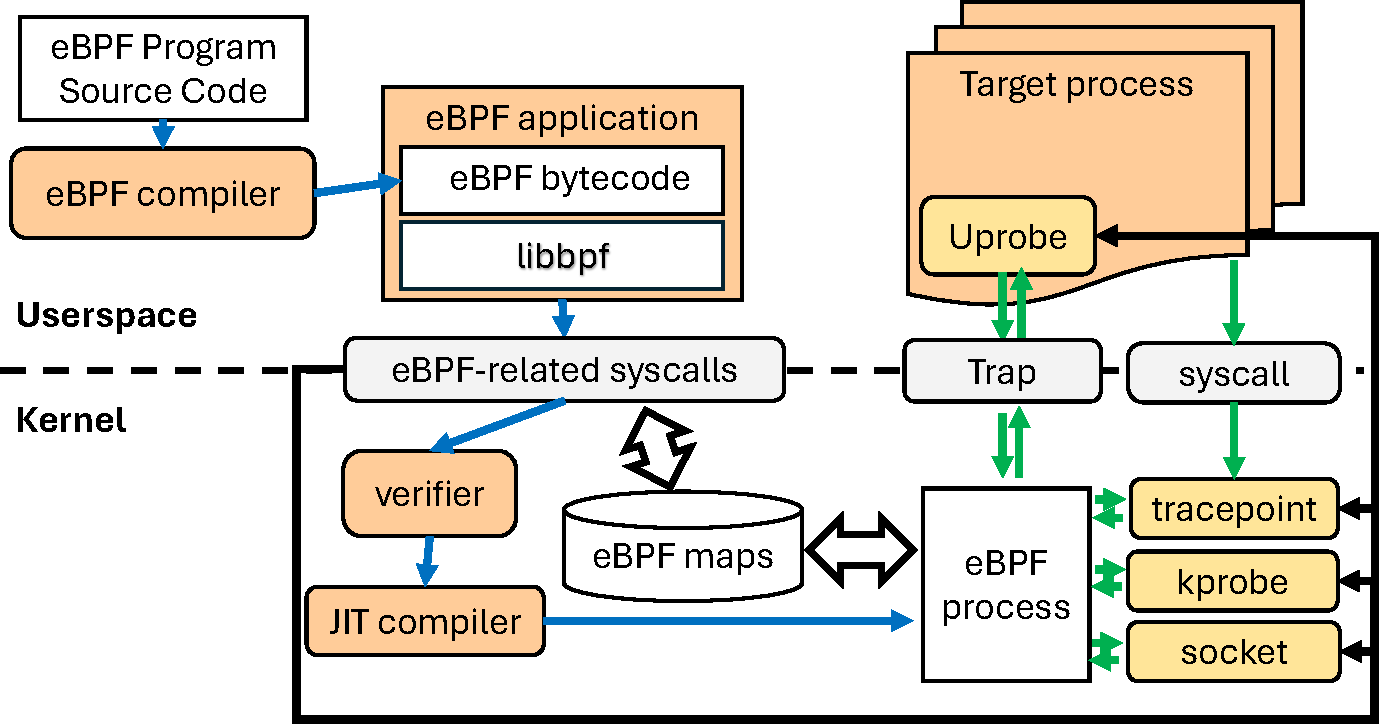
\includegraphics[width=\columnwidth]{img/ebpf-diagram-cropped.pdf}
\caption{eBPF Design.  Blue arrows show execution flow when compiling and loading an eBPF application. Green arrows show execution flow when an eBPF extension executes.  White arrows with black outline indicate components that interact with eBPF maps.}\label{fig:eBPF-design}
\end{figure}

Our goal is to build a comprehensive, dynamic, safe, and efficient extension framework.  Our approach centers around two guiding design principles.  First, we seek to leverage the success and industry clout of the existing eBPF ecosystem.  To this end, we will {\em maintain compatibility} with applications and extensions built for the current state of the art eBPF framework.  As described above, eBPF satisfies many of the design constraints, but degrades comprehensiveness and efficiency by executing userspace extension logic in the kernel.  To remedy this, as the second guiding principle, we seek to run user extensions entirely in userspace {\em without requiring kernel involvement}, even as they inter-operate with other eBPF extensions in the kernel or elsewhere in the system. %\arq{One downside of how these are presented is that they don't point back to the design goals established in the previous section} \yusheng{I think the four princeples, comprehensive, dynamic, safe, and efficient are for the general extension systems. Since we choose eBPF, we want our new extension system still supports a large ecosystem exists in the world, and can run complex, real world extension applications. So this is the main design constrains for our extension system besides the four lists before.} \yusheng{They are mainly for "keep comprehensive, dynamic, safe, and efficient, and also able to run real-world non-trival extension tasks in real world production systems"}

In the remainder of this section, we first provide further background
on the current eBPF ecosystem (\cref{sec:challenges:eBPF-background}).
Then, we outline the challenges that arises when extending eBPF
execution into userspace (\cref{sec:challenges:details}).


\subsection{eBPF Background} \label{sec:challenges:eBPF-background}

This section describes the current eBPF framework. \Cref{fig:eBPF-design} shows the  critical components of the ecosystem and how their interaction.  We discuss the three main phases of interacting with eBPF: writing an eBPF program, loading an eBPF program, and executing an eBPF program.


\subsubsection{Writing eBPF Applications}

An eBPF application consists of two components: (1) the code that will run in the context of the larger system to perform tracing or customization, called the {\em extension} or {\em eBPF program}; and (2) the userspace control plane application that loads one or more extensions and later communicates with them (e.g., to extract and/or analyze data), called the {\em eBPF application}.  

The user writes an eBPF program (eBPF Program Source Code), by specifying a set of functions that will execute in an event-based manner.  Each function will execute when the attached program reaches a configured event, called a \emph{hook point}, specified using a symbolic name (e.g., a function name in the kernel or a path to an executable and function name for user applications).  There are many possible hook points from general (\texttt{uprobe}s, \texttt{kprobe}s, etc.) to specific (XDP~\cite{vieira2020fast}, seccomp~\cite{seccomp-ebpf}, etc.).  The most general hook points are \texttt{uprobe}s and \texttt{kprobe}s, which support extending any userspace or kernel instruction, respectively.  eBPF programs can use a rich set of {\em eBPF helper functions} for reading memory, obtaining process information, etc.  Importantly, the eBPF framework provides helper APIs so that programs can store state in buffers called {\em maps} to communicate with other extensions, the control plane eBPF application, the external system, or a future invocations of the same eBPF extension.  Extensions are typically written in C, with hook points specified as section names that will be interpreted by the eBPF application at load time using a library such as libBPF.

The user passes their eBPF program to an eBPF compiler (e.g., \texttt{clang}), which produces an ELF binary containing the program's extension logic (\ie its functions) represented in eBPF bytecode, their associated hook points as an ELF binary, and information about the maps for the eBPF progrma. 

An eBPF application forms the control plane of a distributed set of extensions.  It is responsible for loading, communicating with and coordinating extensions, and, as such, can be very complex.  Due to the breadth and complexity of these applications, compatibility with the current eBPF ecosystem (our first guiding design principle) is critical.

%% A user writes an eBPF program (eBPF Program Source Code).  The user expresses each of the extensions that they wish to add to the system as a separate function. They annotate the hook point for each extension using the syntax \mintinline{c}{SEC("<type>/<name>")} indicating that the function should be executed when the program reaches the hook point \mintinline{c}{name} of probe type \mintinline{c}{type} (\eg \texttt{kprobe}, \texttt{uprobe}, \texttt{uretprobe}, etc.).  The user can leverage a rich set of eBPF helper functions to help with many tasks, including access eBPF maps, read memory, get process information, etc.  \Cref{code:example} provides a simple but realistic eBPF program that finds which go-routine is accepting TCP connection and report the event to userspace eBPF application. The uprobe program gets the relation between go-routine ID and thread ID, store it into the hash map. The kprobe program is triggered on tcp connect events, get the related go-routine ID from hash map and report the event to userspace with ring buffer.

%% The user passes their eBPF program to an eBPF compiler (e.g., \texttt{clang}), which produces eBPF bytecode for the user's extensions. The bytecode consists of the program's extension logic (\ie its functions), maps and their associated hook points as an ELF binary.  

\subsubsection{Loading and Attaching eBPF Programs}

Regardless of whether an eBPF program will extend the kernel or a userspace application, the eBPF application utilizes kernel system calls to create any required maps, load each eBPF program, and attach each program to the specified hook point.  This is typically accomplished via a library, such as libBPF.

When a user loads an eBPF program, the kernel ensures that the eBPF bytecode is safe to execute using static analysis.  Namely, the in-kernel verifier checks if the eBPF bytecode is memory and type safe by checking the type and memory offset of each memory dereference in the bytecode using metadata released with each kernel called the BPF Type Format (BTF).  Next, the verifier ensures that the bytecode terminates by ensuring that all loops have a constant bound and are not recursive. The verifier also validates that there are no hardware exceptions in the eBPF bytecode by checking each instruction.  For example, it checks for divisions by unknown scalars to ensure that an extension cannot cause a divide-by-zero exception.  Lastly, the bytecode verifier ensures that the extension does not leak resources by ensuring that all allocated resources (e.g., ring buffer memory) are released on all program paths.

%The purpose of the verifier is to protect the system (kernel or userspace process) from a misbehaving extension.  However, while it does protect against some common mistakes, the verification is not sufficient to protect from an extension that purposefully performs customization or misuses helpers~\cite{hotos-untenable}.  The verifier does not protect the extension from the system.  However, userspace extensions are protected from the application they are attached to by nature of running in kernel context (discussed next). \arq{While this is all true, I'm wondering if it is totally worth bringing up here, given that we don't have an answer to the concern.} \yusheng{I think maybe we can try to simplify some of the verifier part here?}

Once the verifier is satisfied with the extension bytecode, the kernel compiles it into native code with an in-kernel just-in-time (JIT) compiler.  When instructed to do so via a system call, the kernel attaches the compiled extension program to a hook point.
%There are many possible hook points that an extension can be attached to ranging from general (\texttt{uprobe}s, \texttt{kprobe}s, etc.) to specific (XDP~\cite{xdp}, seccomp~\cite{seccomp-ebpf}, etc.).  The most general hook points are \texttt{uprobe}s and \texttt{kprobe}s, which allow attachment to any userspace or kernel instruction, respectively.  
When attaching an eBPF program to these hook points, the kernel modifies user or kernel code by adding software breakpoints (\ie \texttt{int 0xcc}) that will trap when executed.\footnote{In the kernel, some {\texttt kprobe}s are
optimized to use non trapping instructions.}


%% When the user wishes to execute their extension, they use an existing toolchain (e.g., \texttt{libbpf}) to load the eBPF bytecode.  The toolchain interacts with a number of bpf-related system calls (\eg \mintinline{c}{bpf}, \mintinline{c}{perf_event_open}) to load the extension into the system.  The bpf-related system calls perform three main tasks.  First, some of the eBPF system calls initialize maps for the eBPF program to use. Second, some of the eBPF system calls instrument the actual hook points (e.g., \texttt{uprobe}s, \texttt{kprobe}s, etc.) required by the eBPF program.  The instrumentation adds software breakpoints (\ie \texttt{int 0xcc}) for userspace hook point, and uses trampolines (\ie \texttt{jmp} instructions) for kernel space hook points.  Finally, some of the eBPF system calls validate the eBPF byte code. These calls pass the eBPF bytecode for the user's execution logic to an eBPF verifier.  One important note: the current eBPF ecosystem \emph{does not} verify userspace extensions (\ie those that attach to \texttt{uprobe} and \texttt{uretprobe} hook points).
%% \yusheng{Might be better to describe as "does not ensure userspace extensions don't break userspace process." because it does verify the uprobe eBPF don't break kernel, like infinity loop or access kernel memory wrong.}

%% The verifier uses static analysis to ensure that the eBPF bytecode is safe to execute.  Namely, the verifier checks to see if the eBPF bytecode is memory and type safe by checking the type and memory offset of each memory dereference in the bytecode by consulting metadata released with each kernel called the BPF Type Format (BTF).  Next, the verifier ensures that the bytecode terminates by ensuring that all loops have a constant bound, are not recursive.  The verifier validates that there are no hardware exceptions in the eBPF bytecode by checking each instruction.  For example, it checks for divisions by unknown scalars to ensure that an extension cannot cause a divide-by-zero exception.  Lastly, the bytecode verifier ensures that the extension does not leak resources by ensuring that all allocated resources (e.g., ring buffer memory) are released on all possible program paths.

\subsubsection{Executing an eBPF Program}

After the eBPF program is loaded and attached, it will be invoked as the system executes.  Specifically, when the system encounters a trap, the kernel will execute the associated extension.   Note that the extension program runs in kernel context regardless of the hook point location. For userspace hook points, invoking the eBPF program incurs at least two context switches (one to the kernel and one back to userspace), and is often even more expensive as the system also must emulate the logic of the instruction replaced by the software breakpoint.  This significant overhead  prevents the existing eBPF framework from meeting the performance design constraint.

% As the eBPF program runs, it may utilize helper functions to read and modify the system's state and use eBPF maps to save system state across extension invocations, allowing extensions at different hook points and/or the eBPF application to cooperate to solve the user's problem. 

%% After the eBPF program is loaded, the system begins executing.  The kernel provides a Just-in-time (JIT) Compiler that takes the verified eBPF bytecode as input and compiles it as necessary to the native architecture of the machine.  The system executes the eBPF bytecode logic each time it reaches a configured hook point.  The eBPF bytecode read and modify the system's state and use eBPF maps to save system state across extension invocations, allowing extensions at different hook points to cooperate to solve the user's problem.  While the trampoline technique used for kernel hook points provides efficiency, the software breakpoint mechanism for \texttt{uprobe} or \texttt{uretprobe} does not.  Each userspace extension requires executing a trap.  This incurs at least two context switches (one to the kernel and one back to userspace), often even more as the system must execute the logic of the instruction located at the software breakpoint, which comes with high overhead.
%% L

\subsubsection{DeepFlow Example}
\begin{figure}[t]
\centering
\begin{minted}{c}
BPF_RINGBUF_OUTPUT(rb, 1 << 4);
BPF_HASH(goroutines, u64);

SEC("uprobe/go-server-http:runtime.casgstatus")
int uprobe_runtime_casgstatus(struct pt_regs * ctx) {
  void *gp = ctx->ax;
  u64 goid;
  if (bpf_probe_read_user(&goid, sizeof(goid),
                          gp + GOID_OFFSET) == 0) {
    u64 thread = bpf_get_current_pid_tgid();
    bpf_map_update_elem(&goroutines, &thread, 
                        &goid, 0);
  }
  return 0;
}

SEC("kprobe/tcp_v4_connect")
int BPF_KPROBE(tcp_v4_connect, struct sock* sk) {
  u64 thread = bpf_get_current_pid_tgid();
  u64 *goid_p = bpf_map_lookup_elem(&goroutines, 
                                    &thread);
  u64 data[2];
  data = bpf_ringbuf_reserve(&rb, sizeof(*data), 0);
  if (goid_p && data) {
      BPF_CORE_READ_INTO(&data[0], sk, 
                         __sk_common.sk_rcvbuf);
      data[1] = *goid_p;
      bpf_ringbuf_submit(data, 0);
  }
  return 0;
}
\end{minted}
\vspace{-0.5cm}
\caption{A simplified eBPF implementation of DeepFlow. 
\label{code:example}}
\vspace{-0.5cm}
\end{figure}
We describe a subset of the extensions for DeepFlow (see \cref{sec:motivation:examples}); \cref{code:example} provides the example code.  The program tracks the initial value of a socket option, the size of the receive buffer, to see if it is related to poor socket performance.  The program attaches logic on the userspace code that schedules \texttt{go-routine}s (\mintinline{c}{runtime.casgstatus}) to track the \texttt{go-routine} \texttt{ID} corresponding to each kernel thread.  It identifies the size of the receive buffer (\texttt{sk\_rcvbuf}) of each tcp socket at connection time (\mintinline{c}{tcp_v4_connect}).  It  outputs the \texttt{go-routine ID} and the \texttt{sk\_rcvbuf} value to aring buffer; the eBPF application correlates this output with request-level tracing to identify if poor request performance is correlated with initial \texttt{sk\_rcvbuf} values (this code is not shown).


\subsection{Userspace eBPF Challenges} \label{sec:challenges:details}

Our approach resolves the efficiency and comprehensively limitations of eBPF by executing userspace extensions directly in the target process without requiring kernel involvement.  Moreover, our approach maintains compatibility with applications and extensions built for eBPF.  This approach exposes three challenges: 

\paragraph{A New eBPF runtime for the eBPF Ecosystem} eBPF applications use a vast ecosystem of tooling, including a set of eBPF-related system calls, helper functions, eBPF maps, and a eBPF JIT compiler, which must evolve to execute in userspace.  Our approach must be compatible with this current ecosystem to ensure comprehensiveness.  This includes supporting eBPF-related system calls, providing similar eBPF helper functions for userspace extensions, providing comprehensive eBPF maps, and providing a JIT compiler for executing eBPF code in userspace.  Prior works on userspace eBPF (ubpf~\cite{ubpf} and rbpf~\cite{rbpf}) support userspace eBPF JIT compilers, but do not handle the other issues. 

\paragraph{Trap-free Userspace Extensions} Injecting a userspace extension in eBPF is simple: replace program bytes with software breakpoints (\ie traps).  However, traps require kernel involvement, violating the goal of kernel-free userspace extension execution.  Trap-free extensions in an arbitrary userspace process is difficult, especially to support extensions on \texttt{syscall tracepoints}, which must instrument \emph{every} \texttt{sysenter} instruction in the program.  

\paragraph{Safety} Executing userspace extensions exposes the system to two safety problems.  First, the kernel's verifier assumes that eBPF bytecode executes over the kernel's runtime and ecosystem, it cannot be used to ensure that a buggy extension cannot crash the system.  Second, executing the extension within the target process renders it susceptible to compromise by a subverted application.  Preventing such attacks requires (1) that the target process cannot modify the extension logic and (2) that the memory used by the eBPF extension can be shared across userspace and kernel extensions without being read/written by the target process.


%% \sys{} resolves the efficiency and comprehensively challenges of the current eBPF ecosystem by executing userspace extensions directly in the target process.   The approach is conceptually simple, but it exposes a number of critical challenges: 

%% \paragraph{A New eBPF Runtime and Ecosystem} The existing eBPF runtime can only be executed within the kernel; it does not work in a userspace context. \yusheng{ubpf and rbpf exist}  This includes the kernel's JIT Compiler as well as the many eBPF helper functions that the runtime provides to simplify eBPF program development.  Running an eBPF extension from userspace requires a new userspace runtime and new userspace helpers to fill these gaps. \yusheng{I think you might remove this paragraph because it's not challenge}
%% \yusheng{I think we have discussed this before? The challenge here is not the eBPF runtime itself, because there already exist 2 userspace jit eBPF runtime, ubpf and rbpf. it's also easy to implement the helpers.}
%% \yusheng{The actually challenge is that 1. Our goal is provided compatible with existing eBPF toolchains and libraries, but the current eBPF loading process is complex, requires a sets of different syscall, include bpf, perf event open, mmap, epoll, open, close... syscalls, it's typically requires thousands of syscall executions to load and control all the eBPF programs in a eBPF application like deepflow. So the loader is complex and requires 4000 lines. If we don't provide compatibility to the toolchains, then it's impossible to run the large eBPF application like deepflow or even smaller bcc tools like sslsniff.}
%% \yusheng{Another challenge is about eBPF maps. currently the eBPF ecosystem already has userspace jit implement, but not userspace maps implementation, especially we want to have shared maps between userspace and kernel, and shared maps between different userspace. We need to implement a lot of data structures in shared memory. This is critical for the execution of eBPF programs. I have discussed that in ppt.}
%% \yusheng{The attach complexity and safety complexity is exist.}

%% \yusheng{Suggested:}
%% \paragraph{A New eBPF Runtime for current Ecosystem} The existing eBPF applications like deepflow and bcc tools need a set of system call and hundreds to thousands of interactions with kernel to load their eBPF programs and maps. We need to provide compatibility with current bpf related syscalls to reuse the existing eBPF ecosystem and toolchains. There are already JIT compilers like ubpf and rbpf, but running eBPF programs in userspace still requires new eBPF maps implementation provide comprehensive, which is shared between kernel and userspace or different userspace processes to fill these gaps.

%% \paragraph{Attaching to an arbitrary program} The current eBPF ecosystem's logic for attaching to a userpsace program is a simple implementation that replaces program bytes with software breakpoints.  However, attaching to an arbitrary userspace process is significantly more difficult, especially to support extensions on \texttt{syscall tracepoints}, which need to instrument \emph{every} \texttt{sysenter} instruction in the program. 

%% \paragraph{Safety} Executing userspace extensions exposes the system to two safety problems.  First, the kernel's verifier assumes that eBPF bytecode executes over the kernel's runtime and ecosystem, so \sys cannot use it to ensure that a buggy extension cannot crash the system.  Second, executing the extension within the target process renders it susceptible to compromise by a subverted application.  Preventing such attacks requires that \sys{} ensure (1) that the target process cannot modify the extension logic and (2) that the memory used by the eBPF extension can be shared across userspace and kernel extensions without being read/written by the extended process.

